\section{Background}\label{sec:background}

\subsection{Constrained Application Protocol}
CoAP is a lightweight web transfer protocol specialized for use with constrained devices and is currently a Proposed Standard RFC made by The Internet Engineering Task Force (IETF) \cite{Inter93:online}. CoAP is designed for M2M communication which includes the device-to-cloud connectivity model.
CoAP runs over the UDP transport protocol which helps keeping the message overhead small and thereby limits the need for fragmentation.
CoAP can be reliable even though UDP is used as transport protocol because CoAP handles the reliability and congestion control by enabling the message type Confirmable (CON). 
The use of confirmable message means that it requires an acknowledgement from the receiver of the message. 
To limit the number of simultaneous unacknowledged and confirmable messages, congestion control is implemented by use of the back-off algorithm.

The message format for CoAP, illustrated in \figurename{\ref{fig:msgformatcoap}}, contains among others a header with a length of 4 bytes. 
%a token for identifying the different requests, CoAP options, and payload. 
\begin{figure}[bht]
	\centering
	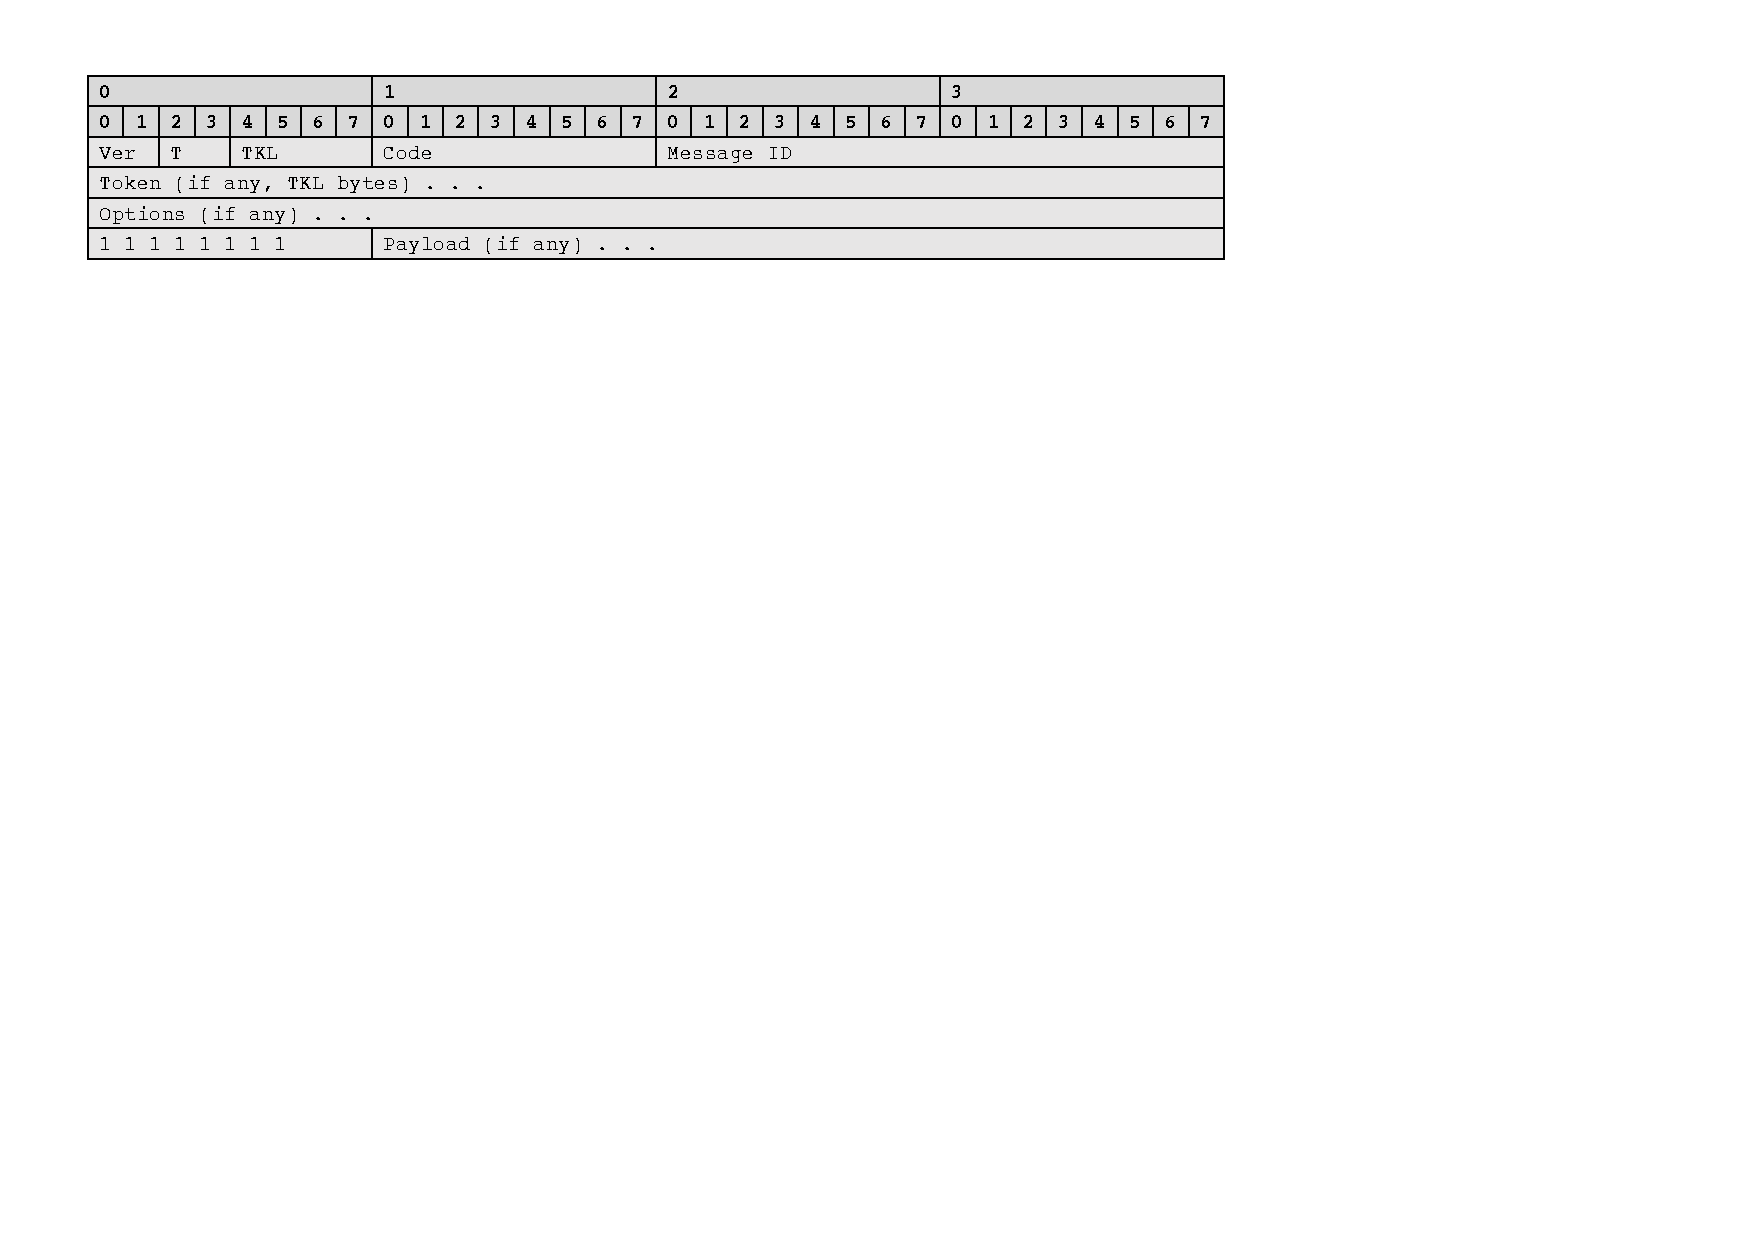
\includegraphics[width=3.5in]{gfx/msgformat-coap}
	\caption{The CoAP header.}
	\label{fig:msgformatcoap}
\end{figure}

The header contains the following fields: 
\begin{list}{-}{}
	\item Version (ver) indicates the version of the CoAP protocol.
	\item Type (T) indicates the type of the message e.g. non-confirmable.
	\item Token length (TKL) indicates the length of Token field.
	\item Code indicates the status of the response or the request method. 
	\item Message ID is an identifier for relating acknowledgements to CON-messages and detection of duplicated messages as well.
\end{list}

CoAP is in many ways similar to HTTP and thus it is easy to convert CoAP messages to HTTP and vice versa. This is normally done by use of a proxy, which for example can be used as a broker between embedded devices and the web. 

%not asynchronous - has to wait for an aknowledged

%For security the Datagram Transport Layer Security (DTLS), which is based on the stream-oriented Transport Layer Security (TLS), is used.

%--UDP can only transfer small amounts of data

\subsection{Constrained Application Protocol over TCP}
CoAP over TCP is an Active Internet-Draft made by IETF. 
In this draft it is proposed to use TCP as a transport protocol instead of UDP.
CoAP over TCP is made for use for certain environments that benefits from using CoAP directly over a reliable communication channel which can easily come through firewalls, provides additional information to NAT, has longer session life, and is able to send requests asynchronously. 

CoAP over TCP is based on the original version of CoAP with some modifications. 
The use of TCP as a transport layer protocol removes the need for handling reliability, congestion control, and other features, which already exist in TCP at the CoAP level.
Since it is not necessary to handle reliability at the CoAP level, all the communication in the CoAP over TCP are by use of non-confirmable (NON) messages and thereby the fields, Type (T) and Message ID, are unnecessary and thus removed from the header. 
The Message ID is also removed because TCP handles duplication detection as well.
Moreover the version (ver) is also removed from the header. The reason for this change is not specified in the draft.

Two new fields are added to the CoAP over TCP header as illustrated in \figurename{\ref{fig:msgformatcoapovertcp}}.
\begin{figure}[bht]
	\centering
	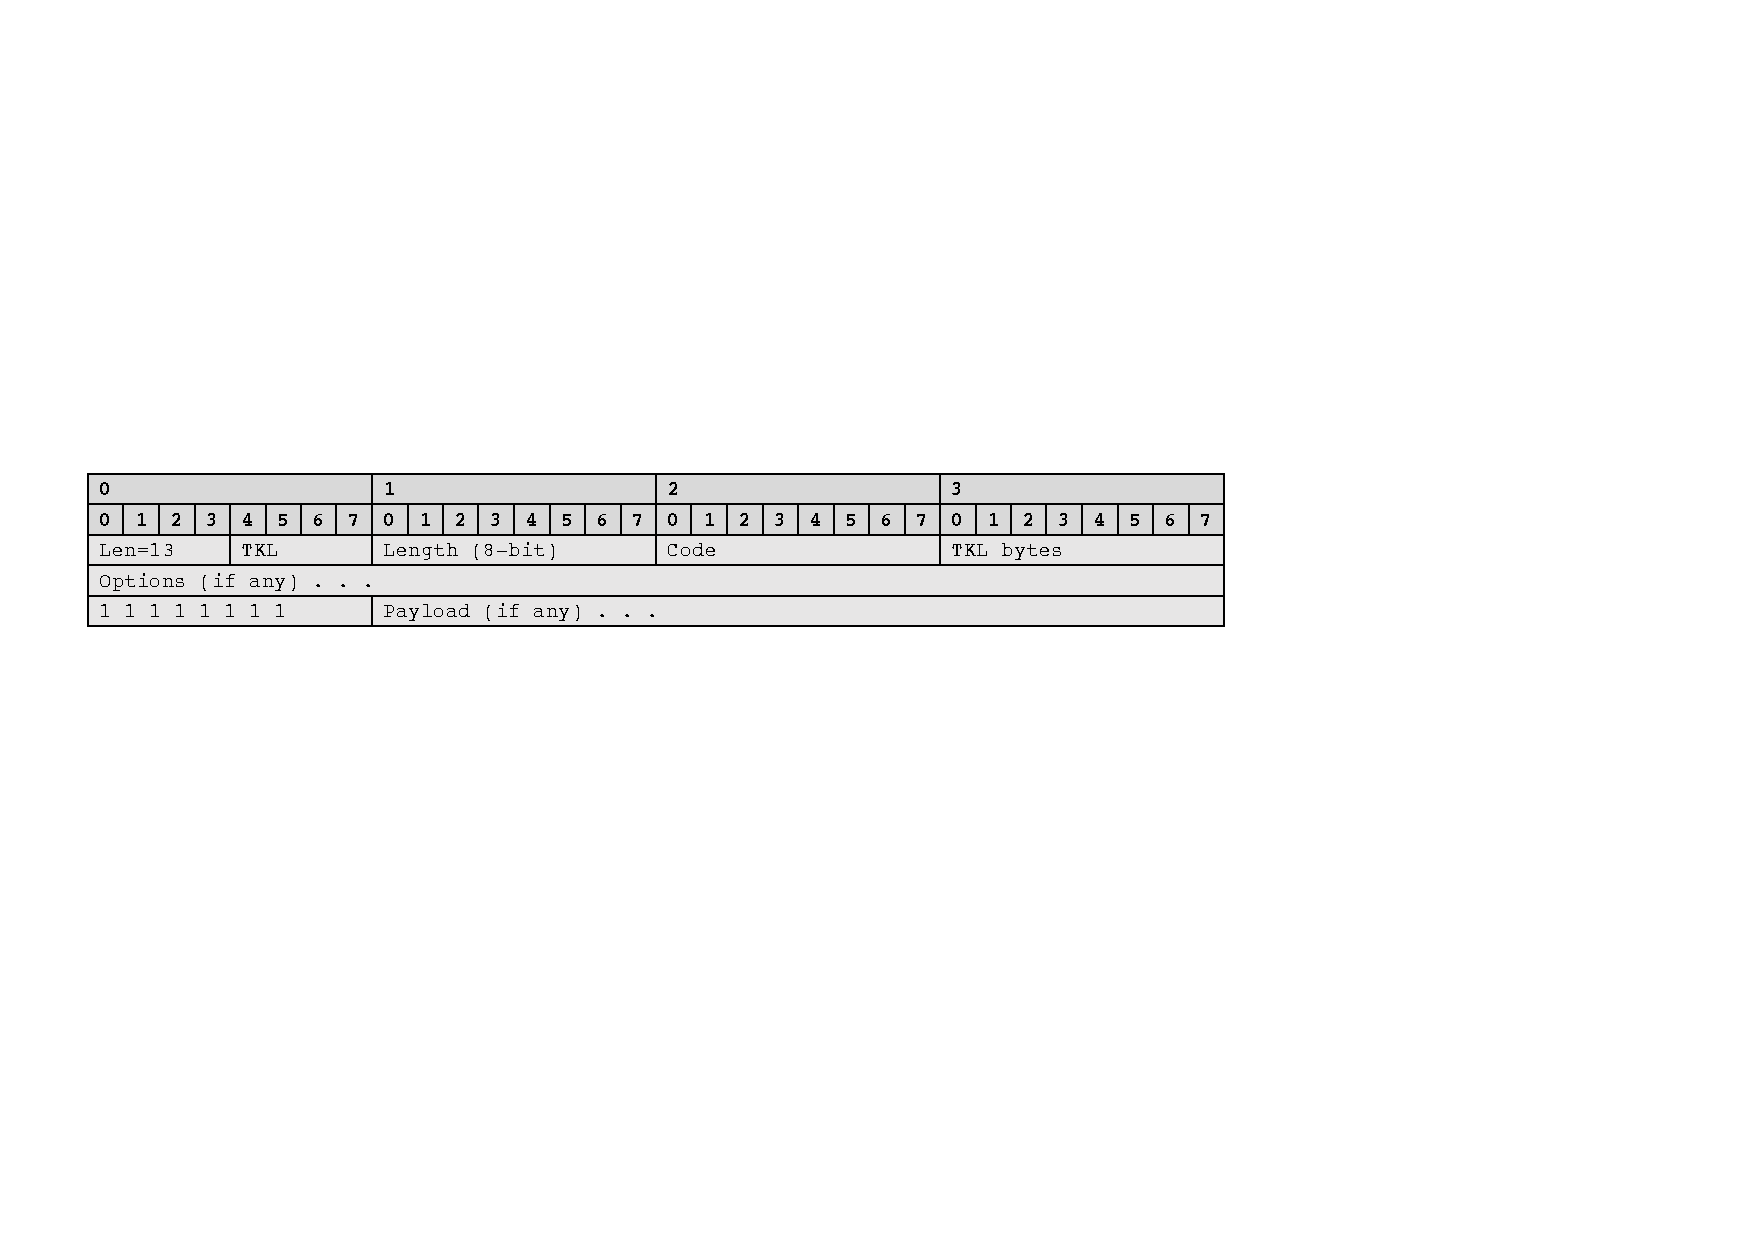
\includegraphics[width=3.5in]{gfx/msgformat-coapovertcp}
	\caption{The CoAP over TCP message format with 8-bit Length in header.}
	\label{fig:msgformatcoapovertcp}
\end{figure}

These fields are, Len and Length, which are used to indicate information about the amount of data sent in form of payload/options.  
This addition was necessary to take advantage of message delimitation supported by TCP.

%The use of TCP as a transport layer also makes it easier to avoid being blocked by firewalls.  
%The use of TCP as a transport layer also enables asynchronous message exchange, which makes it possible to transmit TCP requests simultaneously without the need for waiting for an acknowledgement. 

%TLS
%
%TCP has less risk of being blocked by firewalls than UDP
%No lost packages/data
%Provides additional information about session life to NAT
%Long lifetime
%No need for handling reliability
%(Exchanges messages asynchronously even though it runs TCP)
%TLS
%Is the changes in the header compatible with the current CoAP implementation?
%
%
%Background: Beskrivelse af de to protokoller, forholdsvis kort (undlade detaljer, som ikke er relevant for artiklen)





%\subsection{Middleware as Solution for Interoperability}
%Middleware has proven to be a solution in many environments for ensuring interoperability within distributed systems. In IoT the same way of thinking has been adapted. 
%Several projects in collaboration between big companies are currently developing  middleware solutions for IoT and one of these solutions is IoTivity which supports CoAP as an application protocol.
% 
%In \cite{interoperabilityChallenge} the IoTivity framework is evaluated according to defined requirements among others the connectivity where different connectivity models are evaluated. These connectivity models are device-to-device, device-to-gateway, and device-to-cloud. Results from the evaluation of IoTivity shows that device-to-cloud communication within constrained devices is challenging.
%
%\subsection{Device-to-Cloud}
%Existing solutions for communicating with device-to-cloud are HTTP, MQTT, CoAP...etc.
%
%compare solutions....
%
%
%HTTP 
%
%MQTT



